\documentclass[a4paper]{article}
\usepackage{amsmath}
\usepackage[utf8]{inputenc}
\usepackage{amsmath}
\usepackage{cancel}
\usepackage[portuguese]{babel}
\usepackage{fancybox}
\usepackage{amssymb}
\usepackage{capt-of}
\usepackage{pgfplots}
\usepackage{tikz}
\usepackage{polynom}
\usepackage{adjustbox}
\usetikzlibrary{matrix}
\usetikzlibrary{calc}
\usetikzlibrary{patterns}
\usetikzlibrary{decorations.pathreplacing}

\begin{document}
	
\section*{Exercício 1}\textbf{Das representações gráficas seguintes indique, justificando, as que podem representar funções, indicando, para essas, o domínio e o contradomínio.}	

\begin{center}
	\adjustbox{valign=t}{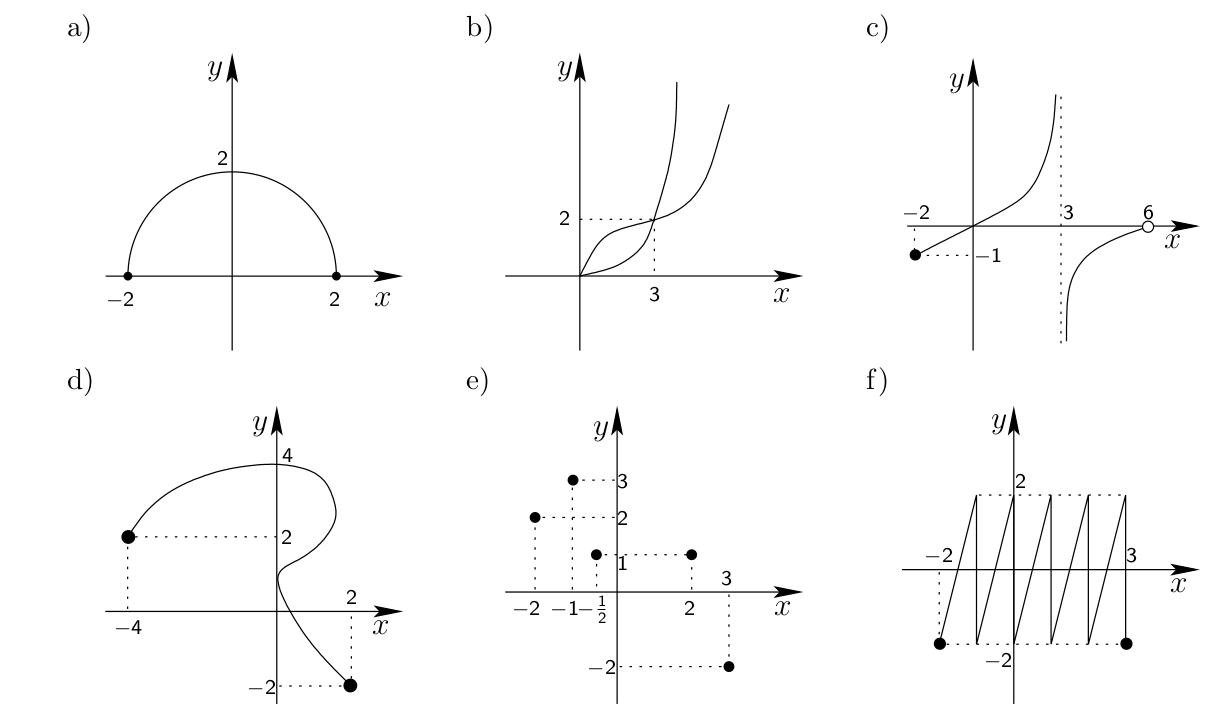
\includegraphics[width=1.3\textwidth]{images/ficha7ex1.png}}
\end{center}
\text{As funções são $\it{a,c}$ e $\it{e}$.}
\[D_{a}=\left[-2,2\right]\]
\[D'_{a}=\left]0,2\right[\]
\[D_{c}=\left[-2,3\right[\cup \left]3,6\right[\]
\[D'_{c}=\left]-\infty,+\infty\right[=\mathbb{R}\]
\[D_{e}=\{-2,-1,-\frac{1}{2},2,3\}\]
\[D'_{e}=\{-2,1,2,3\}\]
\section*{Exercício 2}
\textbf{Considere a função real de variável real definida por $f(x)=- \frac{3x-1}{2}$.}
\subsection*{a)}\textbf{ Verifique se o ponto $\left(-\frac{1}{2} , \frac{5}{4}\right)$ pertence ao gráfico de $\it{f}$.}
\[f(-\frac{1}{2})=-\frac{3\cdot\left(-\frac{1}{2}\right)-1}{2}=\frac{5}{4}\]
\subsection*{b)}
\textbf{Calcule $f(-\frac{1}{3})$.}
\[f(-\frac{1}{3})=-\frac{3\cdot\left(-\frac{1}{3}\right)-1}{2}=1\]
\subsection*{b)}
\subsection*{c)}
\textbf{Resolva a condição $f(x)>-3$ e indique o significado geométrico desta condição.}
\[-\frac{3x-1}{2}>-3\]
\[\Leftrightarrow x < \frac{7}{3}\]
\text{Para as imagens superiores a $-3$ os objetos são inferiores a $\frac{7}{3}$.}
\section*{Exercício 3}\textbf{Determine o domínio das seguintes funções:}
\subsection*{a)}
\textbf{$f(x)=\frac{1}{x}+5$;}
\[D_{f}=\{x \in \mathbb{R}: x \neq 0\}\]

\subsection*{b)}
\textbf{$f(x)=\frac{x}{x^2+x}$;}
\[D_{f}=\mathbb{R}\setminus \{-1,0\}\]

\subsection*{a)}
\textbf{$f(x)=\frac{\sqrt{1-x}}{\sqrt{9+4x}}$;}
\[D_{f}=\{x \in \mathbb{R}: 1-x \geq 0 \land  9+4x > 0 \}=\left[-\frac{9}{4},1\right]\]

	\section*{Exercício 4}\textbf{Considerere as funções}
\[f(x)=\begin{cases}
	\text{$3$, se $x < 2$,}\\ 
	\text{$x-3$, se $x \geq 2$.}
\end{cases}\] 
e
\[g(x)=\begin{cases}
	\text{$-2$, se $x=-1$,}\\ 
	\text{$-x+3$, se $-1 < x < 3$,}\\
	\text{$-x$, se $3 \leq x < 6$.}
\end{cases}\]

\subsection*{a)}
\textbf{Determine $D_{f}$ e $D_{g}$.}
\[D_{f}=\mathbb{R}\]
\[D_{g}=\left[-1,6\right[\]
\[D'_{f}=\left[1,+\infty\right[\]
\[D'_{g}=\left]-6,-3\right] \cup \{-2\} \cup \left]0,4\right[\]

\subsection*{b)}
\textbf{Represente graficamente cada uma das funções.}

f(x)=
	\begin{tikzpicture}[>=latex]
	\begin{axis}[
		axis x line=center,
		axis y line=center,
		xtick={-7,-6,-5,-4,...,5,6},
		ytick={-7,-6,-5,-4,...,5,6},
		xlabel={$x$},
		ylabel={$y$},
		xlabel style={below right},
		ylabel style={above left},
		xmin=-6.5,
		xmax=8,
		ymin=-6.5,
		ymax=6.5]
		\addplot[domain=2:6] {(\x)-3};
		\addplot[domain=-5:2] {3};
		\draw[dashed] (axis cs:2,0) -- (axis cs:2,-1) -- (axis cs:0,-1);
		\addplot[mark=*] coordinates {(2,-1)};
		\addplot[mark=*,fill=white] coordinates {(2,3)};
	\end{axis}
\end{tikzpicture}

g(x)=
\begin{tikzpicture}[>=latex]
	\begin{axis}[
		axis x line=center,
		axis y line=center,
		xtick={-7,-6,-5,-4,...,5,6},
		ytick={-7,-6,-5,-4,...,5,6},
		xlabel={$x$},
		ylabel={$y$},
		xlabel style={below right},
		ylabel style={above left},
		xmin=-6.5,
		xmax=8,
		ymin=-6.5,
		ymax=6.5]
		\addplot[domain=-1:3] {-(\x)+3};
		\addplot[domain=3:6] {-(\x)};
		\draw[dashed] (axis cs:3,0) -- (axis cs:3,-3) -- (axis cs:0,-3);
		\addplot[mark=*] coordinates {(-1,-2)};
		\addplot[mark=*] coordinates {(3,-3)};
		\addplot[mark=*,fill=white] coordinates {(6,-6)};
		\addplot[mark=*,fill=white] coordinates {(-1,4)};
		\addplot[mark=*,fill=white] coordinates {(3,0)};
	\end{axis}
\end{tikzpicture}

\subsection*{c)}
\textbf{Verifique se alguma das funções é injetiva.}

\text{f(x) é não injetiva pois todos os objetos inferiores a 2 têm a imagem 3.}

\text{g(x) é injetiva.}
\[\forall a,b \in D, a \neq b \implies f(a) \neq f(b)\]

\subsection*{d)}
\textbf{Indique, caso existam, o máximo e o mínimo absolutos de $\it{g}$.}

\text{g(x) não tem máximo nem mínimo absolutos.}

\section*{Exercício 5}\textbf{Estude a paridade das funções:}
\begin{itemize}
	\item \textbf{ par quando, para qualquer $a \in D$, se tem $-a \in D$ e
	$f(-a)=f(a)$;}
	\item \textbf{ ímpar quando, para qualquer $a \in D$, se tem $-a \in D$ e
	$f(-a)=-f(a)$;}
	\end{itemize}
\subsection*{a)}
\textbf{$f(x)=x-4x^2$;}
\[f(-x)= -x - 4x^2\]
\[-f(x)= -x + 4x^2\]
\text{Não é par nem ímpar.}
\subsection*{b)}
\textbf{$f(x)=1-x^4$;}
\[f(-x)= 1-x - x^4\]
\[-f(x)= -x + x^4\]
\[f(x)=f(-x)\]
\text{É par.}
\subsection*{c)}
\textbf{$f(x)=\sqrt[3]{x}-9x^3$;}
\[f(-x)= -\sqrt[3]{x}+9x^3\]
\[-f(x)= -\sqrt[3]{x}+9x^3\]
\[f(-x)=-f(x)\]
\text{É ímpar.}
\section*{Exercício 6} \textbf{Considere os gráficos das funções $\it{f},\it{g},\it{h},\it{i},\it{j},\it{k}: \left]0,1\right[\longrightarrow\mathbb{R}:$}

\begin{center}
	\adjustbox{valign=t}{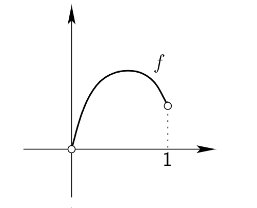
\includegraphics[width=0.5\textwidth]{images/6f.png}} 
	\label{fig:6f}
\end{center}
\begin{center}
	\adjustbox{valign=t}{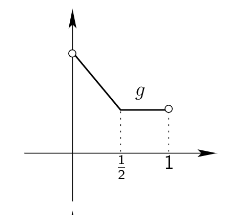
\includegraphics[width=0.5\textwidth]{images/6g.png}} 
	\label{fig:6g}
\end{center}
\begin{center}
	\adjustbox{valign=t}{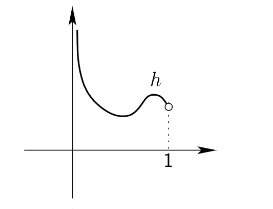
\includegraphics[width=0.5\textwidth]{images/6h.png}} 
	\label{fig:6h}
\end{center}
\begin{center}
	\adjustbox{valign=t}{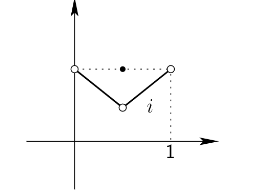
\includegraphics[width=0.5\textwidth]{images/6i.png}} 
	\label{fig:6i}
\end{center}
\begin{center}
	\adjustbox{valign=t}{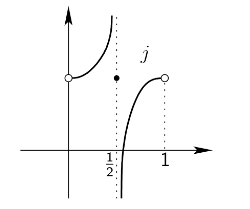
\includegraphics[width=0.5\textwidth]{images/6j.png}} 
	\label{fig:6j}
\end{center}
\begin{center}
	\adjustbox{valign=t}{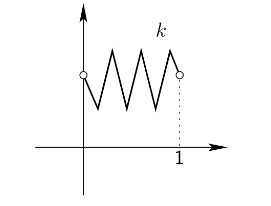
\includegraphics[width=0.5\textwidth]{images/6k.png}} 
	\label{fig:6k}
\end{center}
\subsection*{a)}
\textbf{Indique as funções que têm máximo absoluto.}
\text{$\it{f,i,k}$}
\subsection*{b)}
\textbf{Indique as funções que têm mínimo absoluto.}
\text{$\it{g,h,k}$}
\subsection*{c)}
\textbf{Indique o conjunto dos minimizantes de $\it{g}$.}
\text{$\left[\frac{1}{2},1\right[$}
\subsection*{d)}
\textbf{Indique as funções que são sobrejetivas.}
\text{$\it{j}$}
\subsection*{e)}
\textbf{Indique as funções que são não injetivas.}
\text{$\it{f,g,h,i,k}$}
\subsection*{f)}
\textbf{Indique as funções que não são limitadas.}
\text{$\it{h,j}$}
\subsection*{g)}
\textbf{Indique as funções decrescentes.}
\text{$\it{g}$}
\subsection*{h)}
\textbf{Indique as funções crescentes.}
\text{Não há.}
\subsection*{i)}
\textbf{Indique os intervalos de monotonia de j.}
\[\left]0,\frac{1}{2}\right[,\left]\frac{1}{2},1\right[\]
\end{document}